\documentclass[a4paper,10pt]{article}
\usepackage{graphicx}
\usepackage[utf8]{inputenc}

%opening
\title{Instructivo EyeExperimenter}
\author{Ariel E. Arelovich}

\begin{document}

\maketitle

\section{Requerimientos de conectividad}
El programa EyeExperimenter \textbf{requiere de una conexión a internet sólo para el pedido de reporte}. Es decir el programa es perfectamente capaz de tomar cuantos estudios sean necesarios sin la necesidad de conexión. \textbf{No existe un modo offline u online}. Solo se utiliza la conexión a internet para procesar la información recolectada en los estudios y nada mas. 

\section{Procedimiento para el pedido de informe}

Los reportes se piden desde la pantalla de \textit{Lista de Sujetos}. Para acceder a esta pantalla sólo es necesario prender el programa, seleccionar un doctor e ingresar la contraseña de doctor. Luego se verá la pantalla como se muestra Figura~\ref{fig_lista_sujetos}.

\begin{figure}[!h]
\centering
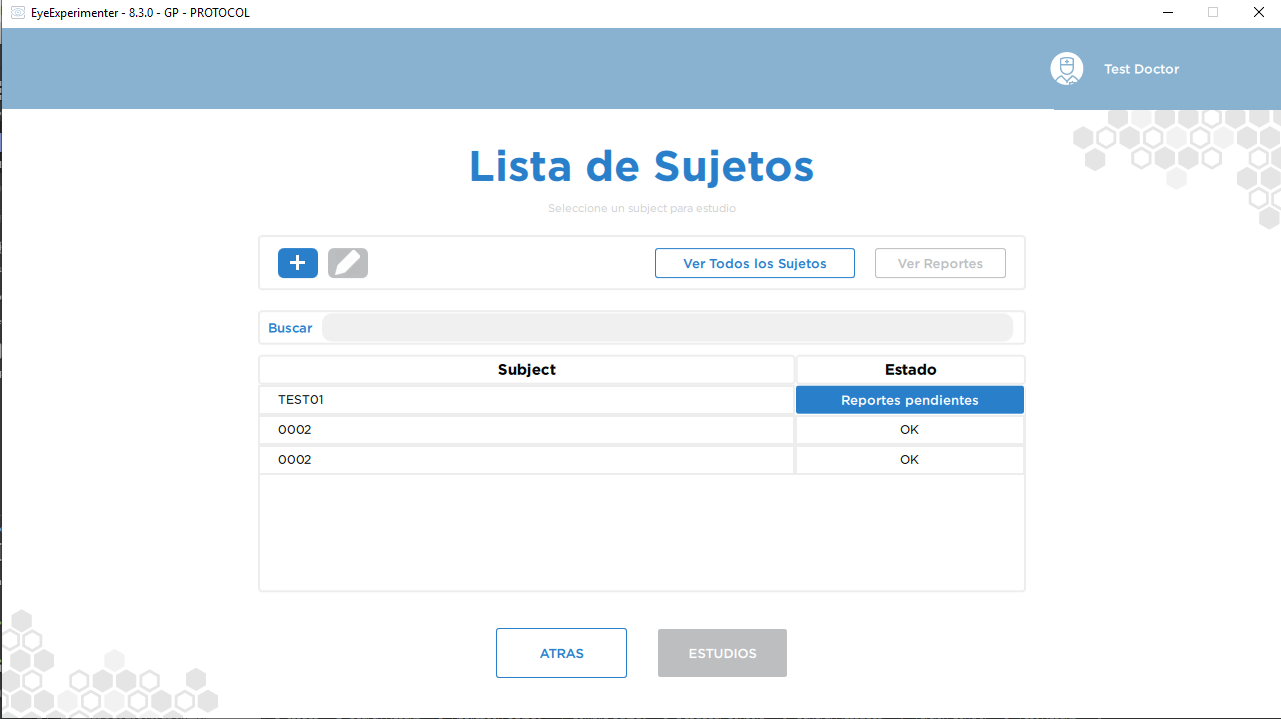
\includegraphics[scale = 0.4]{reportes_pendientes.png}
\caption{Pantalla de \textit{Lista de Sujetos}}
\label{fig_lista_sujetos}
\end{figure}

Todos aquellos sujetos que presenten envaluaciones que puedan ser enviadas a procesar mostrarán un boton azul con las palabras \textit{Reportes Pendientes}. Oprimiendo dicho botón se comienza el proceso de pedido de reporte. 

\begin{figure}[!h]
\centering
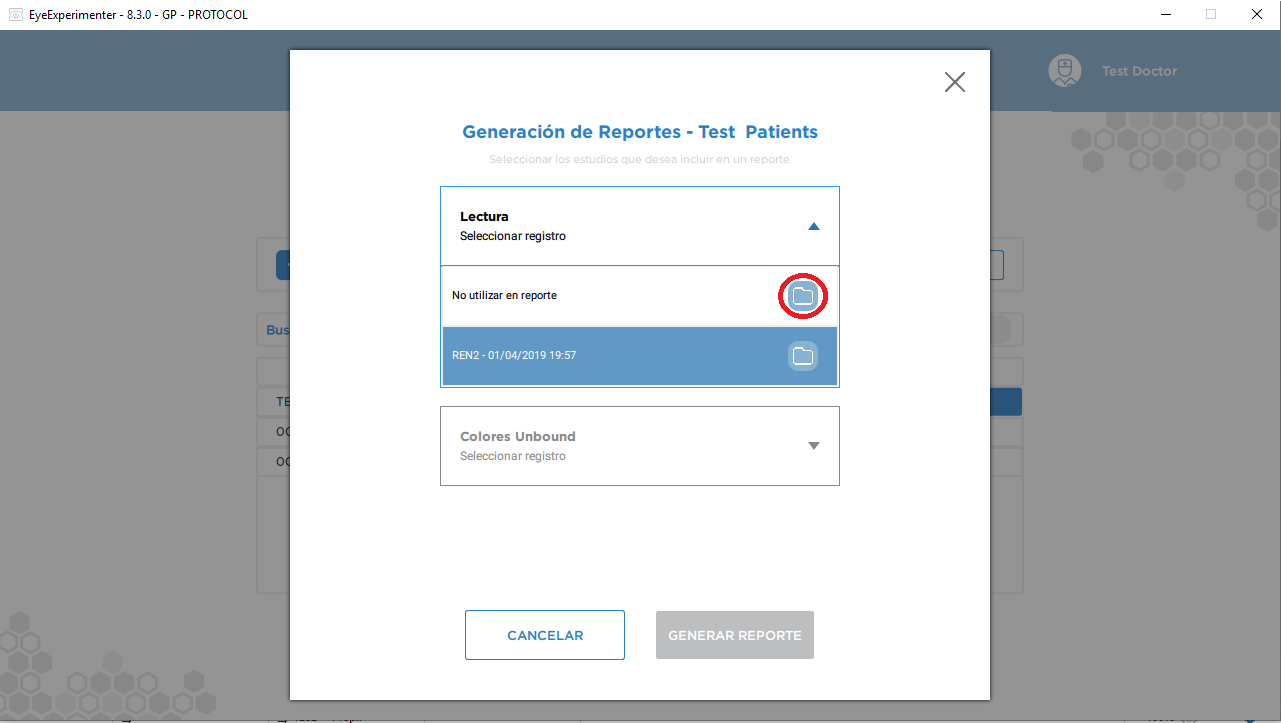
\includegraphics[scale = 0.4]{selectt_first.png}
\caption{Diálogo de \textit{Generación de Reportes}}
\label{fig_rep_gen}
\end{figure}

Al oprimir el botón se abrirá un diálogo como el que se muestra en al Figura~\ref{fig_rep_gen}. En este diálogo se verán tres campos de selección. Cada campo de selección corresponde a un estudio posible: Lectura, Colores Bound y Colores Unbound. La lista de cada campo se compone de los archivos que el programa ha detectado que no han sido enviados a procesar de cada estudio. 

Cuando se oprime un campo de selección se desplegará la lista de posibles archivos a elegir. La opción \textit{No utilizar en reporte} es utilizada si no existe o no se desea enviar a procesar un archivo con un estudio de lectura. Además al lado de cada opción aparece un ícono de una carpeta. Si se oprime este botón, se abrirá otro diálogo pidiendo la confirmación de que se desea eliminar de la lista el archivo. Este proceso se lo conoce como archivar. La información \textbf{no se borra} y permanece en el PC pero no se volverá mostrar para enviar a procesar.

Es posible pedir un informe, con solo tres variantes. Esto se verá reflejado en le botón \textit{GENERAR REPORTE} que cambiará de gris a azul, indicando que está habilitado y por ende puede ser oprimido.
\begin{enumerate}
 \item Se elige solo un archivo de Lectura
 \item Se selecciona la opción \textit{No utilizar en reporte} para el campo de lectura y luego se selecciona uno archivo de colores bound y otro de colores unbound.
 \item Se selecciona un archivo de lectura, otro de colores bound y uno de colores unbound.
\end{enumerate}

La Figura~\ref{fig_all_sel}, muetra el diálogo de \textit{Generación de Reportes} con todos los campos seleccionados. Una vez que se haya realizado la selección de cuales reportes se oprime el botón \textit{GENERAR REPORTE} y la información seleccionada será enviada al servidor para ser procesada y se devolverá un archivo de reporte. Durante este proceso aparecerá un cartel de espera.

\begin{figure}[!h]
\centering
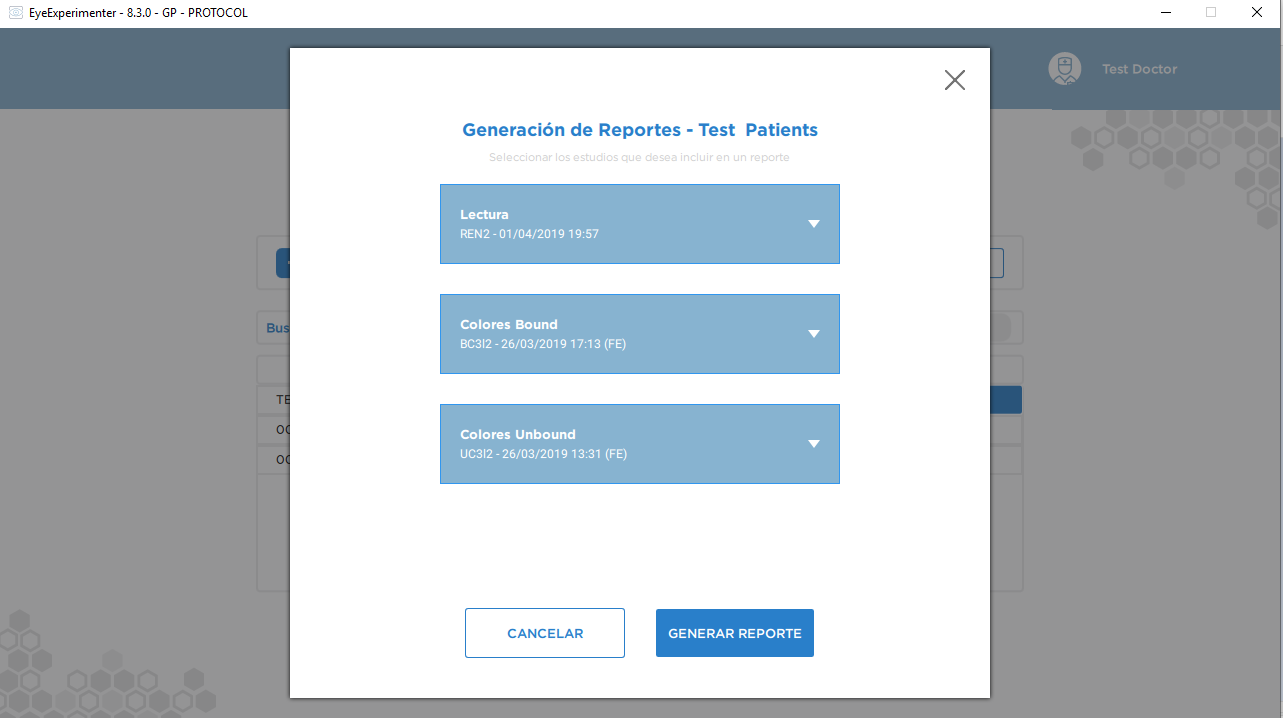
\includegraphics[scale = 0.4]{allselected.png}
\caption{Diálogo de \textit{Generación de Reportes} en el cual todos los campos fueron seleccionados}
\label{fig_all_sel}
\end{figure}

\section{Posibles carteles de error}

La Figura~\ref{fig_freq_err} muestra el cartel de error de frecuencia. Este cartel puede aparecer en dos momentos: al finalizar un estudio o al visualizar un reporte. En el primer caso es por que hubo algún tipo de problema de comunciación con el EyeTracker. Sin embargo \textbf{no es necesario tomar ninguna acción}. El archvio generado puede ser envíado a procesar normalmente y el equipo de ViewMind analizará la calidad de los datos. 

\begin{figure}[!h]
\centering
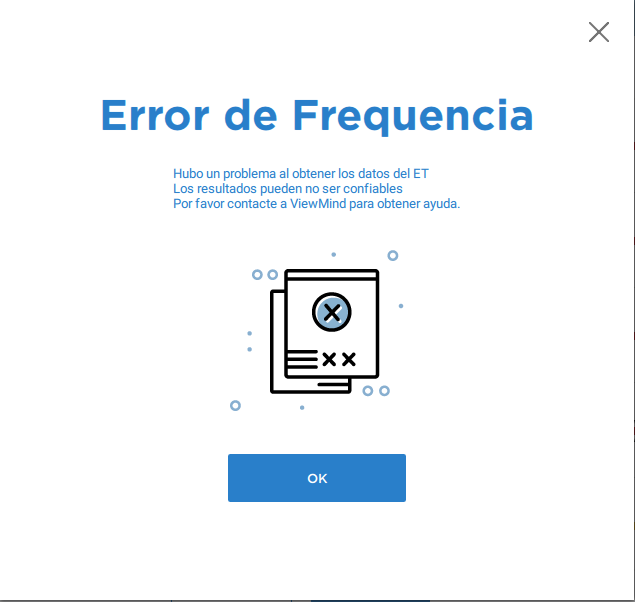
\includegraphics[scale = 0.3]{freq_error.png}
\caption{Diálogo de error de frecuencia}
\label{fig_freq_err}
\end{figure}

La Figura~\ref{fig_comm_err} aparece cuando existe algún problema de conexión y no fue posible la comunicación con el servidor. Cuando esto suceda no se podrán generar reportes. En este caso es necesario revisar la conexión a internet pero el programa sigue siendo completamente funcional. 

\begin{figure}[!h]
\centering
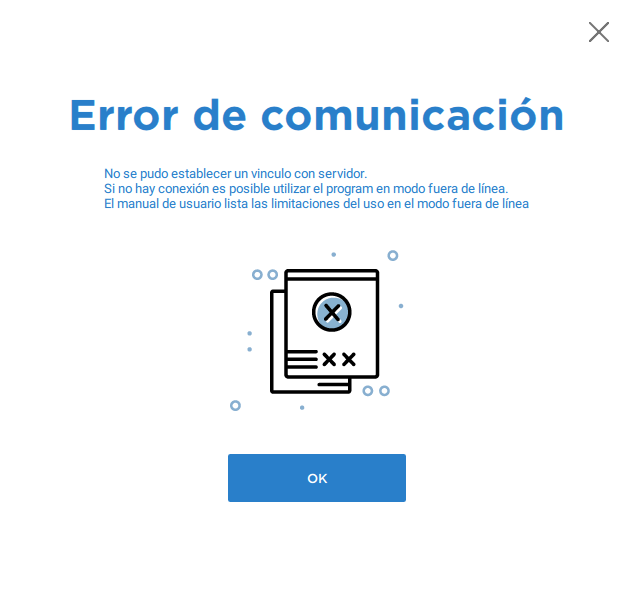
\includegraphics[scale = 0.3]{comm_error.png}
\caption{Diálogo de error de comunicación}
\label{fig_comm_err}
\end{figure}

La Figura~\ref{fig_id_err} se muestra cuando se logra comunicarse con el servidor pero la sincronización de la base de datos local falló. En este caso contactar al equipo de ViewMind. El cartel suele aparecer cuando la conexión a internet no es confiable.

\begin{figure}[!h]
\centering
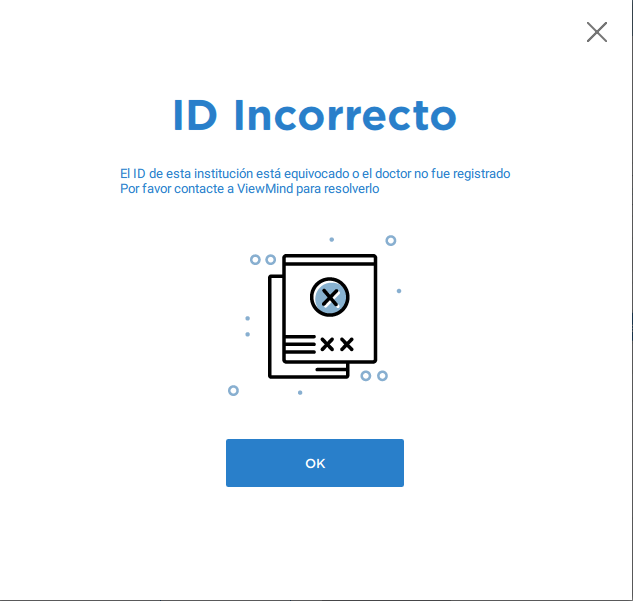
\includegraphics[scale = 0.3]{incorrect_id.png}
\caption{Diálogo de ID Incorrecto}
\label{fig_id_err}
\end{figure}

\section{Eliminar un archivo de estudio}

No es posible, desde el programa, eliminar un archivo de estudio. Sin embargo, si es posible archivarlo, para que no aparezca como una opción en los campos desplegables del diálogo \textit{Generación de Reportes}.

Esto se logra desde el mismo diálogo, oprimiendo el boton con el círculo rojo que se muestra en al Figura~\ref{fig_rep_gen} al lado del archivo que se desea eliminar. Aparecerá un nuevo diálogo para confirmar la acción de Archivar. Una vez confirmada, el archivo desaparecerá de la lista en la cual esta sin enviarse a procesar. 

\end{document}
